\section{Segment Tree}
\index{segment tree}
\index{interval}

% #ifdef hackpackpp

It is often useful to be aware of the range properties of a given array, such as: prefix sums, suffix sums, range minimum queries, range maximum queries, etc.
For simpler problems, a secondary array may suffice to calculate a property like the prefix sum of an array.
The prefix sum calculation only takes $O(n)$ time to perform, and any query thereafter takes only $O(1)$ time.
But any updates to the source dataset will require $O(n)$ time to update the prefix sum calculations.
Frequent changes will quickly show the pitfall of this approach.
This precalculation approach will also not work for finding minimum or maximum values in an arbitrary range.
A segment tree is a data structure for storing information about intervals that can be constructed in $O(n)$ time.
Whenever the source data changes, update times stay low at $O(\log n)$ time.

% #endif

% #ifdef hackpack

A segment tree is represented as an array of a size that is dependent on the dataset it is sourced from.
For a given array of size $n$, a segment tree constructed from it will use up to $2^{\lceil \log_2 (n)\rceil + 1} - 1$ space.
Once built, the structure of a segment tree cannot change.

% #endif

% #ifdef hackpackpp

\begin{figure}[h]
    \centering
    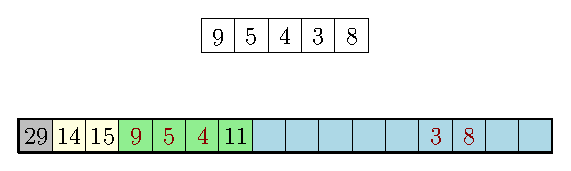
\includegraphics[width=0.6\textwidth]{./structures/segment-tree/source-array}
    \caption{\small The segment tree (bottom) constructed from an array (top) containing five elements.
      The blank entries in the segment tree array are unused.}
\end{figure}

A segment tree is represented as an array of a size that is dependent on the dataset it is sourced from.
For a given array of size $n$, a segment tree constructed from it will use up to $2^{\lceil \log_2 (n)\rceil + 1} - 1$ space.
To properly represent the tree, the root is located at index 0; its left and right children are located at indices 1 and 2 respectively.
To properly recurse through the tree, indices of left and right children can be calculated with $2n + 1$ and $2n + 2$ for left and right children respectively.

Construction of a segment tree begins at the root.
The root node, located at index 0, queries its two children for some property (such as the maximum, the minimum, a range sum, etc\ldots).
Those two children, in turn, query their children.
This process continues until a leaf node, one of the values from the source array, is reached.
The recursive calls return back up the call stack with the parent nodes receiving the information they requested.
These parent nodes record this information and continue returning up the call stack.

As the recursive calls are made, the starting and ending indices that each node represents is passed on.
The left child of a node represents the first half of the section of the dataset the parent represents.
The right child of a node represents the remaining right half.
More precisely, if the parent node represents values between and including a starting index, $a$, and ending index $b$, then the left child will represent values between and including $a$ and $a + \frac{b - a}{2}$.
The right child will represent values between and including $a + \frac{b - a}{2} + 1$ and $b$.
When $a$ and $b$ are equal, a leaf node has been reached, and its value is simply stored at the appropriate index in the segment tree.
Due to the static nature of arrays, once built, the structure of a segment tree cannot change.

\begin{figure}[h]
    \centering
    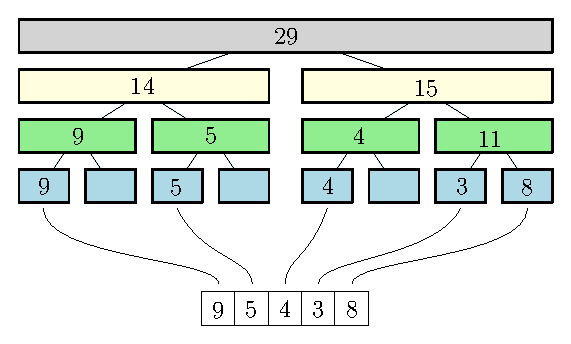
\includegraphics[width=0.6\textwidth]{./structures/segment-tree/array-tree}
    \caption{\small The segment tree visualized in a tree-like format.
    The leaves of the tree are values from the original dataset.}
\end{figure}

% #endif

% #ifdef hackpack

\acmlisting[label=Segment Tree Reference Code, caption=Segment Tree Reference Code]{./structures/segment-tree/segment-tree.cpp}

% #endif


% #ifdef hackpackpp

Generally, a segment tree supports two operations: update and query.
The update operation will account for changes to values in the source dataset.
It is even possible to implement a range update operation to change an entire range of values.
The query operation allows for fast retrieval of segment information.
In the case of the prefix sum, the update operation will modify the tree's nodes such that it will contain correct information after changes, and the the query operation can return a sum for values in an arbitrary range.

\subsection{Applications}

\begin{itemize}
    \item range sums in a frequently changing dataset
    \item range minimum/maximum queries
\end{itemize}

\subsection{Example Contest Problem: Coming and Going}

Farmer John is considering expanding the cows' barn, but he would first like to learn just how many of his cows spend any given time of day in the barn.
In consideration of expanding the cows' barn, Farmer John decided to see just how many of his cows spent any given time of day in the barn.
To do so, he installed motion sensors on each entryway/exit to the building.
These sensors are able to detect both the entry and exit of a warm-blooded being.
This, coupled with his cows' tags, allows him to monitor the movements of specific cows.

The night after the full day in which the sensors were installed, Farmer John sat down to do what he thought was some straightforward analysis, but quickly realized that he was in over his head with only mental math.
He dusts off his old Commodore 64 and begins tabulating the data that he has collected.
Among this data are the times that individual cows were inside the barn.
\textit{While} he enters these times into the computer for each cow, Farmer John wants to see how many cows were inside the barn during a specific time range.

Help him figure out how many cows were inside the barn during specific time ranges as he (slowly) tabulates the data.

\subsubsection{Input Format}

\begin{itemize}
    \item Line 2: A single integer, $C$, representing the number of cows Farmer John has data on.

    \item The following lines are placed in $C$ groups, each describing the movements of a single cow, detailed as follows:
    \begin{itemize}
        \item A single line containing a single integer, $k$, representing the number of time ranges to follow that the cow was present in the barn.

        \item $k$ lines with two distinct integers representing times between which a cow was present in the barn.
        The first number is guaranteed to be strictly less than the second number.
        \item A single line containing two integers $t_1$ and $t_2$ representing times between which the maximum number of cows seen in the barn simultaneously should be reported since the last cow's data was added.
        As usual, with time ranges, the range $t_1$ to $t_2$ includes $t_1$ and all hours leading up to, but excluding $t_2$.
    \end{itemize}
\end{itemize}

\subsubsection{Sample Input}

\acmlisting[label=Coming and Going Sample Input, caption=Coming and Going Sample Input]{./structures/segment-tree/problems/coming-and-going/coming-and-going.in}

\subsubsection{Output Format}

$C$ lines indicating the maximum number of cows seen in the barn in a single hour after adding data for the 1\textsuperscript{st}, 2\textsuperscript{nd}, \ldots, $C$\textsuperscript{th} cow.
Each should appear on its own separate line formatted as given in the sample output.

\subsubsection{Sample Output}

\acmlisting[label=Coming and Going Sample Output, caption=Coming and Going Sample Output]{./structures/segment-tree/problems/coming-and-going/coming-and-going.out}

\subsubsection{Sample Solution}

% #endif

\acmlisting[label=Coming and Going Sample Solution, caption=Coming and Going Sample Solution]{./structures/segment-tree/problems/coming-and-going/coming-and-going.cpp}

% #ifdef hackpackpp

\subsubsection{Lessons Learned}

\begin{itemize}
    \item The data the segment tree keeps track of can easily be changed with a few small modifications to the build, update, and query operations.
\end{itemize}

% #endif
